
\section{Case study}
\label{sec:sysml}
To illustrate our approach, we take an example water tank inspired by \cite{AmalioPCW16}. According to the I/O dependency information between FMUs, the architectural model for water tank is constructed using SysML. The aim of using SysML is to design the architecture of the system with a more high-level modelling language. It helps to show the components and their connections.

%\subsection{Case Study: Water Tank}
The water tank system is our running example as shown in Fig.~\ref{tankfig}. A source of water flows into the water tank whose water flows into the drain. The source is controlled by a valve; when the valve is open, the water flows into the water tank. The valve, managed by a software controller, is opened or closed stochastically or depending on the water level. There are three various water tank systems depending on various connections between controller, valve and tank. 
\begin{figure}[htbp]
	\centering	{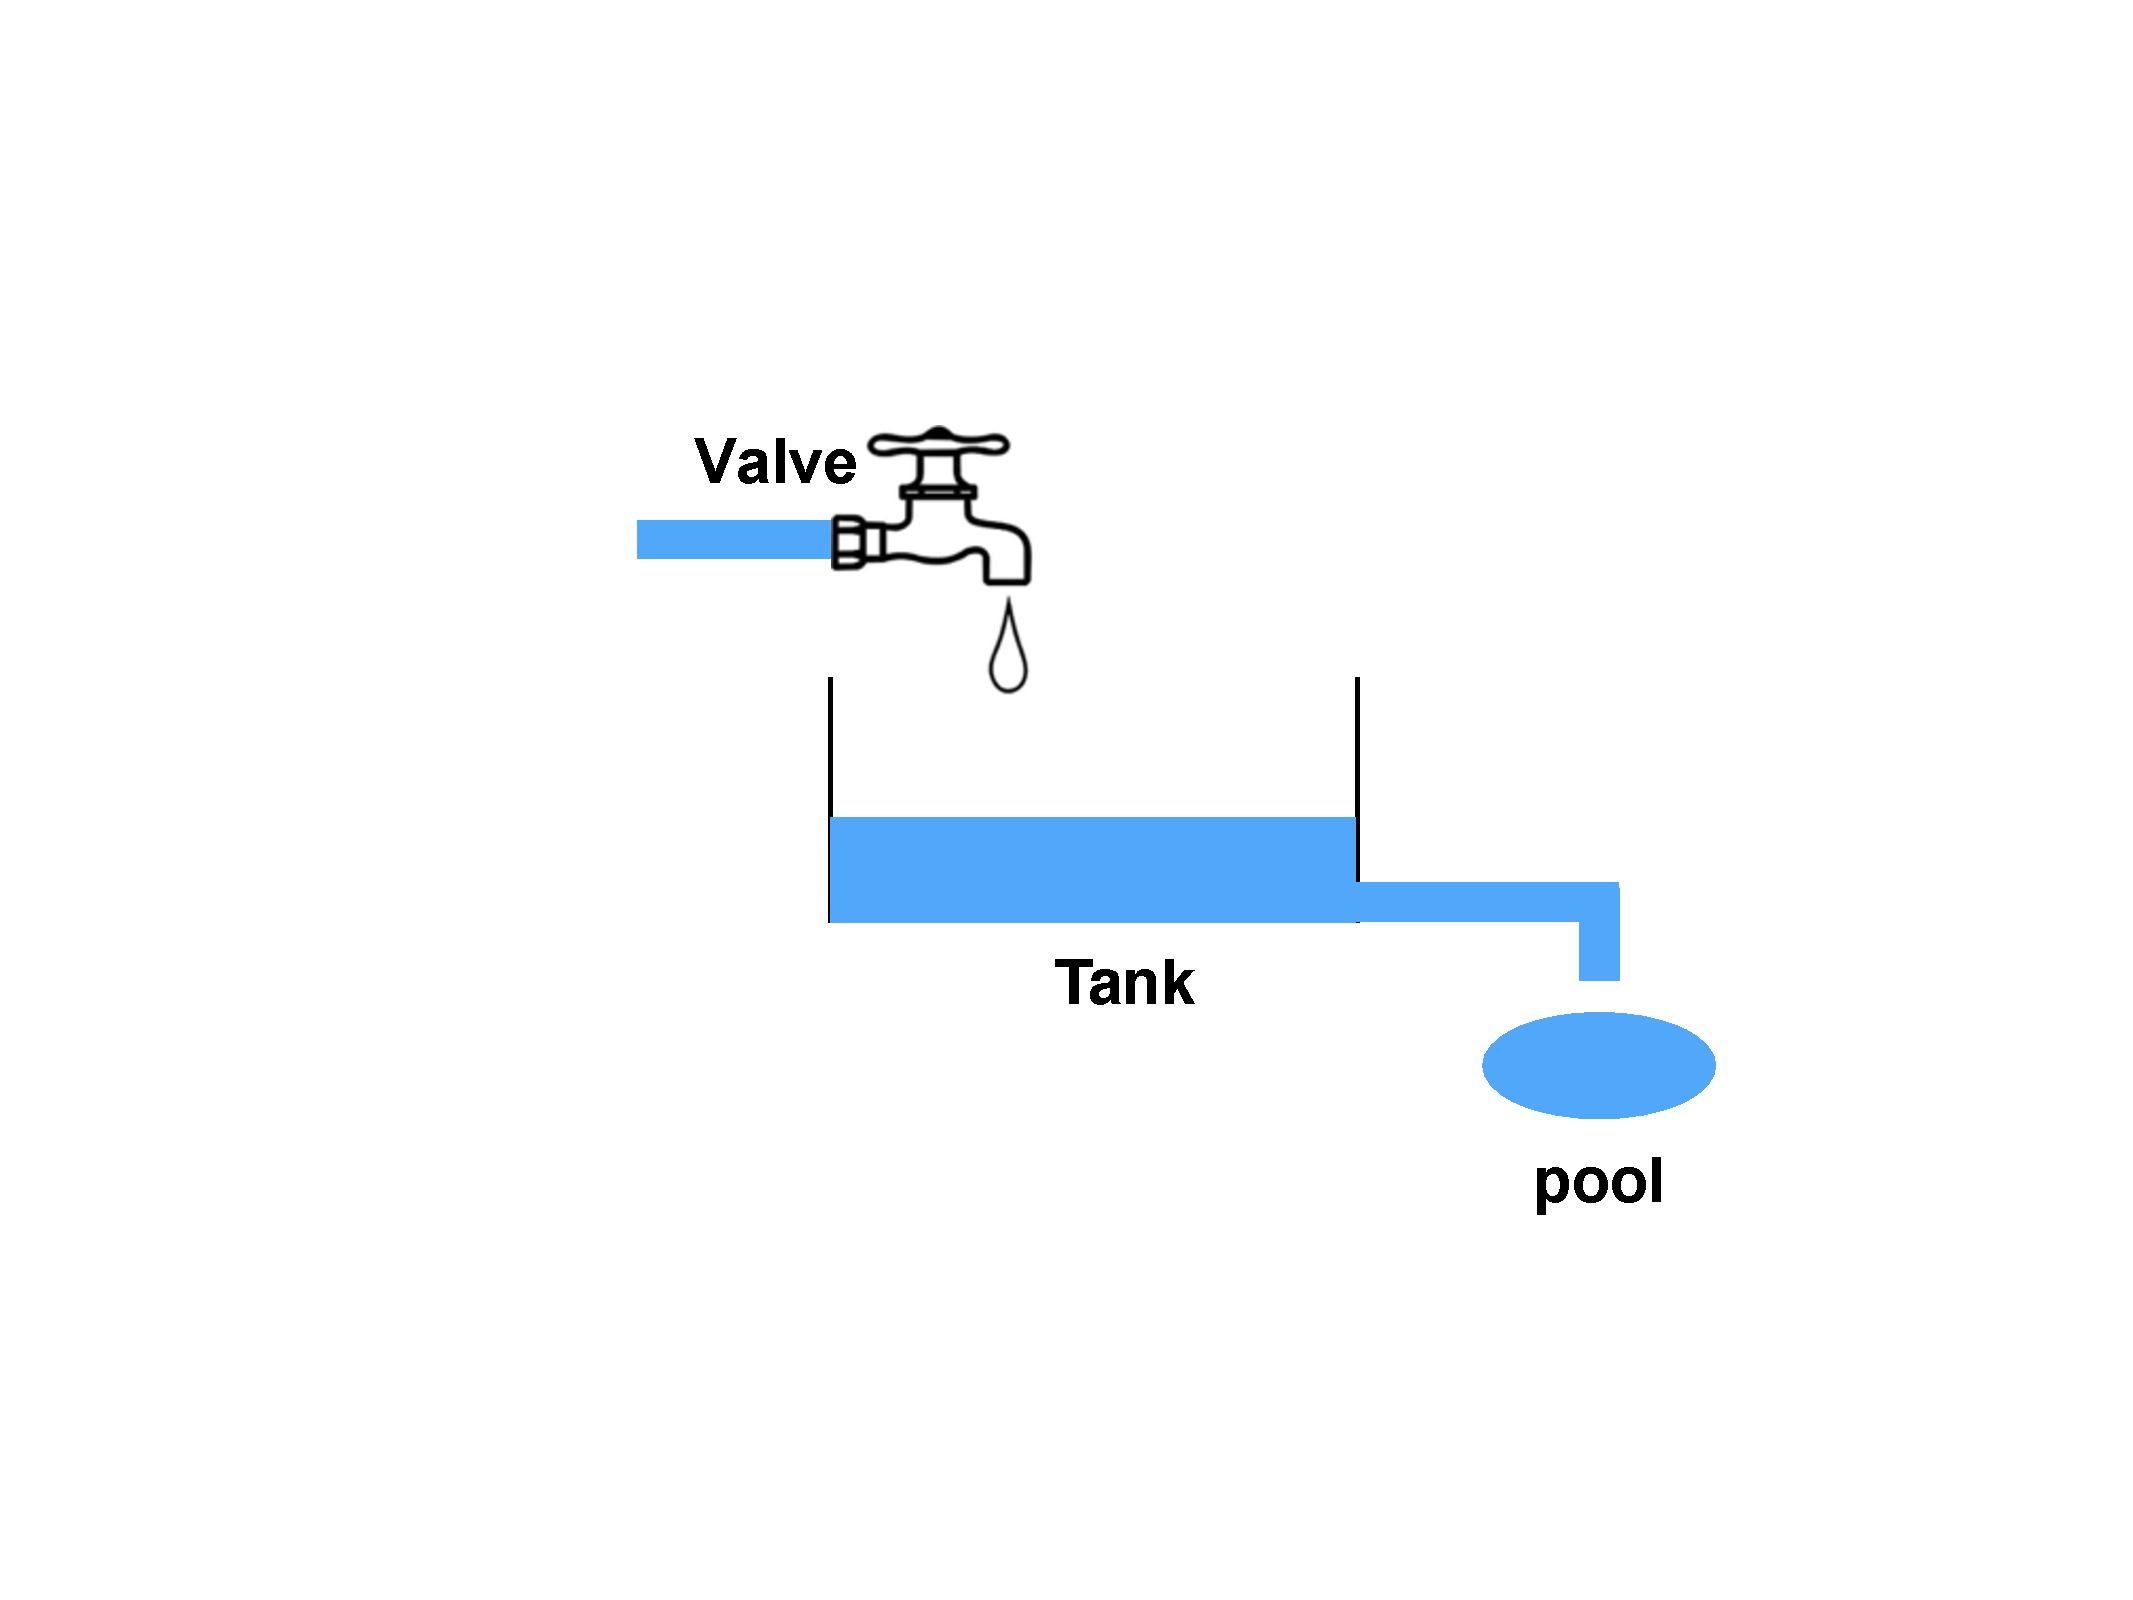
\includegraphics[width=2.2in,height=1.5in]{fig/tank-fig.pdf}}
	\caption{Water tank system.}
	\label{tankfig}
\end{figure}
\subsection{Architecture Modelling in SysML}
SysML is a general purpose domain-specific language (DSL) \cite{SemerathBHSV17} for model-based systems engineering (MBSE) \cite{Dori16}, which is originated as an initiative of the International Council on Systems Engineering (INCOSE) \cite{Pepper2015International} in January 2001. The SysML \textit{Block Definition Diagram} (BDD) describes the system blocks and their features (structural and behavioural). The \textit{Connection Diagram} (CD) describes the internal structure of blocks. The ports of blocks are connected by the connector. The I/O dependence of blocks describes the communication between blocks. SysML block diagrams are usually used to model the architecture of systems.

Fig.~\ref{myad} shows the SysML BDD for the water tank system. The system consists of three blocks, i.e., \emph{Valve}, \emph{Tank} and \emph{Controller}, in which \emph{Valve} and \emph{Tank} are physical components. \emph{Controller} is the cyber component. Each component has its own input and output. For instance, the input interface of \emph{Valve} is named as \emph{vin}, which is used to input the \emph{Open-Closed} signal. 
\begin{figure}[htbp]
	\centering	{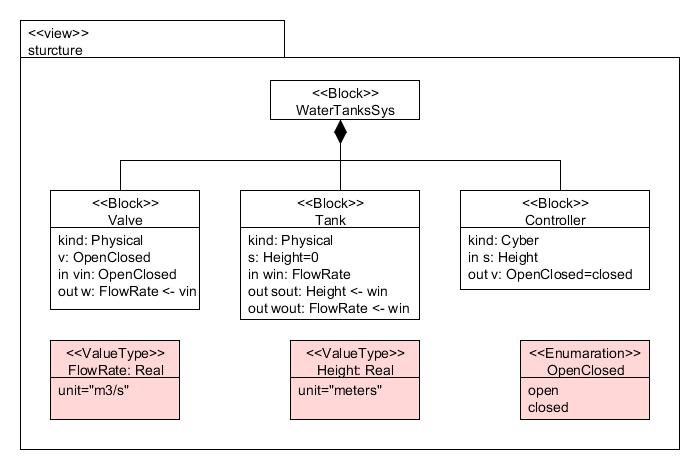
\includegraphics[width=3.2in,height=2.3in]{fig/AD.jpg}}
	\caption{SysML BDD for water tank.}
	\label{myad}
\end{figure}

Fig.~\ref{cd} shows the connection diagram for the system. There are three cases for connections. The first case is that the system has one valve, one controller and one tank. The controller sends stochastic signals to control the valve on/off leading to various rate of water flow. The second case is that the signal from the controller is affected by the water level of the tank. The last case is on the basis of the first case and adds another \emph{waterTank2} which is affected by the flow rate of the \emph{waterTank1}.

\begin{figure}[htbp]
\centering{
		\subfigure[Connection case 1]{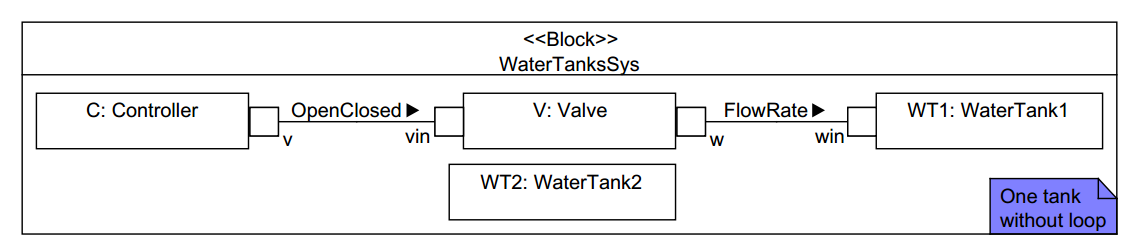
\includegraphics[width=3.2in,height=0.8in]{fig/CD1.png}
			\label{cd1}}
		\hfil
		\subfigure[Connection case 2]{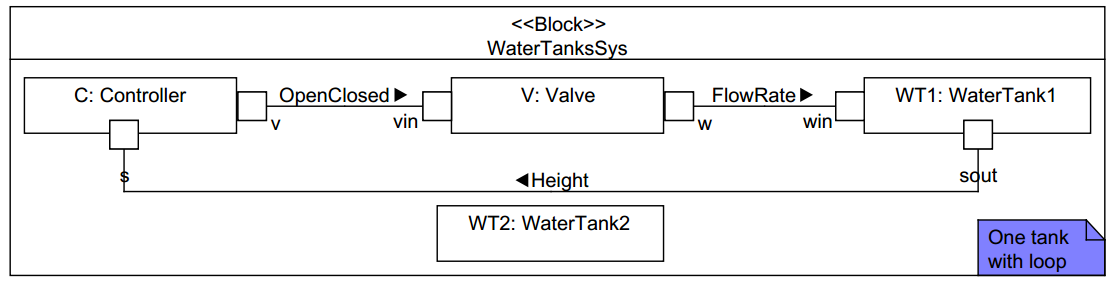
\includegraphics[width=3.2in,height=0.8in]{fig/CD2.png}
			\label{cd2}}
		\hfil
		\subfigure[Connection case 3]{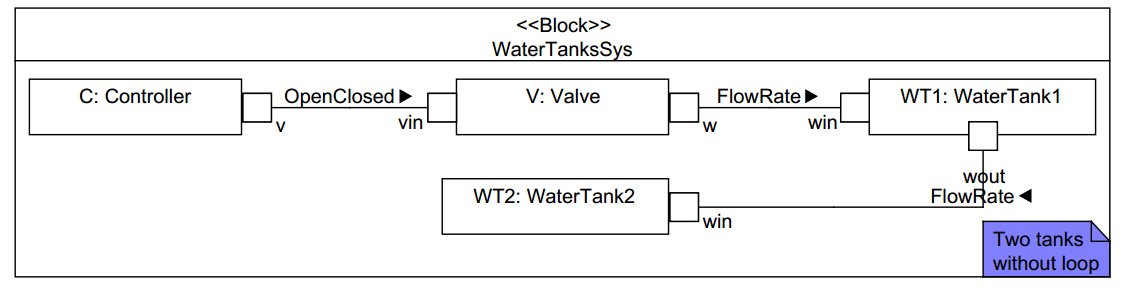
\includegraphics[width=3.2in,height=0.8in]{fig/CD3.png}
			\label{cd3}}
	\caption{SysML connection diagram for water tank.}
	\label{cd}
	}
\end{figure}
The SysML BDD shows the blocks of system and SysML CD shows the connection between blocks. In next section, we abstract each block as a FMU, and obtain the connection between FMUs based on the SysML CD.

\subsection{The FMUs Connection of Water Tank}
Fig.~\ref{fmu-con} is the FMUs and FMUs connection of water tank system. There are three connection cases between the FMUs according to the SysML CD in the previous section. The first case contains three FMU components (\emph{Controller}, \emph{Valve} and \emph{Water tank1}) and two channels ($v \_ vin$, $w \_ win$) as shown in Fig.\ref{fmu-con1}. The \emph{Controller} and \emph{Valve} are connected with channel $v \_ vin$. The \emph{Valve} and \emph{Water tank1} are connected with channel $w \_ win$. The second case is shown in Fig.\ref{fmu-con2}, there could be a channel $sout \_ s$ between \emph{Water tank1} and \emph{Controller}, which means the water level of \emph{Water tank1} affects the control strategy of the \textbf{controller}. Fig.~\ref{fmu-con3} shows the third case, there could be another \emph{Water tank2}, the \emph{Water tank1} and \emph{Water tank2} are connected by the channel $w \_ out$. 
\begin{figure}[htbp]
\centering{
		\subfigure[Connection case 1]{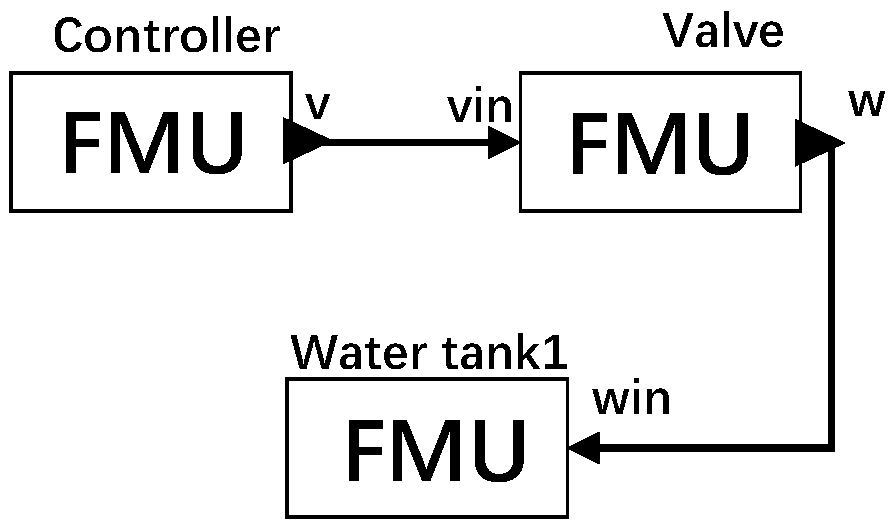
\includegraphics[width=1.0in,height=0.6in]{fig/fmuc1.png}
			\label{fmu-con1}}
		\hfil
		\subfigure[Connection case 2]{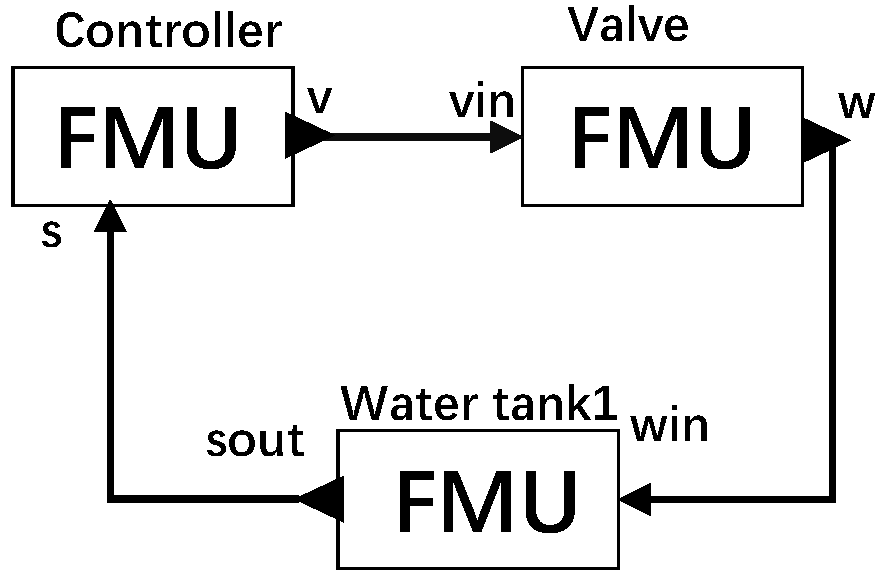
\includegraphics[width=1.0in,height=0.6in]{fig/fmuc2.png}
			\label{fmu-con2}}
		\hfil
		\subfigure[Connection case 3]{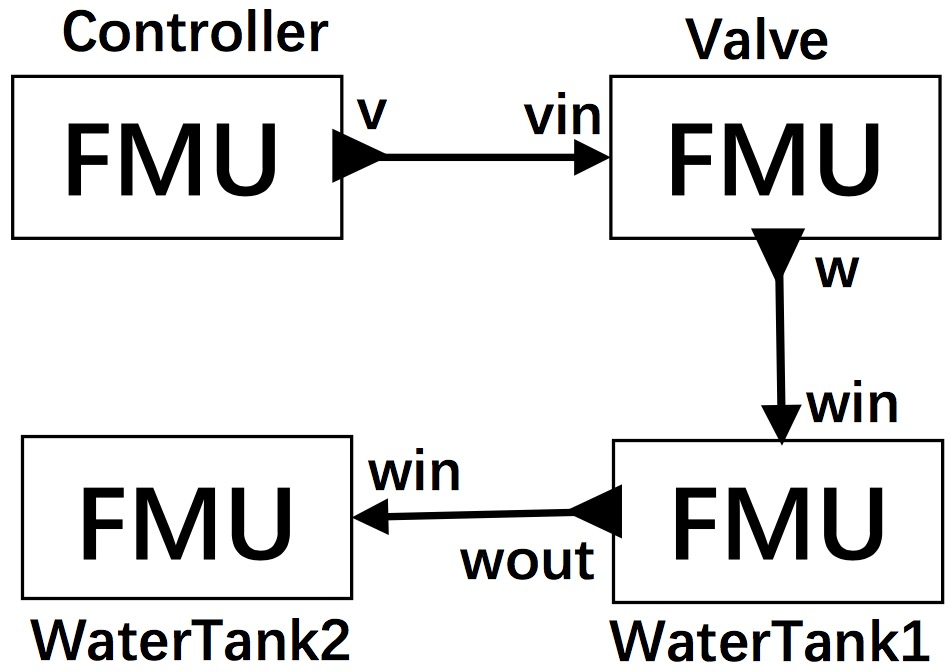
\includegraphics[width=1.0in,height=0.6in]{fig/fmuc3.png}
			\label{fmu-con3}}
	\caption{FMUs connection of water tank.}
	\label{fmu-con}
	}
\end{figure}
How can we assure the correctness of the architecture models? We attempt to verify it with model checking based on timed automata. More details of verification process can be found in the next section.